\documentclass{acm_proc_article-sp}

\usepackage{cite}
\usepackage{graphicx}
%\usepackage[cmex10]{amsmath}
%\usepackage{amssymb}
%\usepackage{array}
\usepackage{url}
\usepackage{listings}

\lstdefinestyle{FortranLike}{float,frame=lines,language=Fortran,commentstyle=\ttfamily,basicstyle=\ttfamily}
\lstdefinestyle{CLike}{float,frame=lines,language=C,commentstyle=\ttfamily,basicstyle=\ttfamily}
\lstdefinestyle{NoFloatCLike}{frame=lines,language=C,commentstyle=\ttfamily,basicstyle=\ttfamily}

\begin{document}

\title{Locally-Oriented Programming: A simple programming model for stencil computations}

\numberofauthors{4}

\author{
% 1st. author
\alignauthor
Craig E Rasmussen\\
       \affaddr{Los Alamos National Laboratory}\\
%       \affaddr{CCS-7, MS B287}\\
       \affaddr{Los Alamos, NM 87545}\\
       \email{crasmussen@lanl.gov}
% 2nd. author
\alignauthor
Matthew J. Sottile\\
       \affaddr{Galois, Inc.}\\
%       \affaddr{421 SW 6th Ave. Suite 300}\\
       \affaddr{Portland, OR 97204}\\
       \email{mjsottile@computer.org}
% 3rd. author
\alignauthor
Dan Nagle\\
       \email{dannagle@verizon.net}
% 4th. author
\alignauthor
Soren Rasmussen\\
       \affaddr{Utah State University}\\
       \email{soren.rasmussen@aggiemail.usu.edu}
}

\maketitle

\begin{abstract}
Some stuff...

%%Emerging GPU architectures for high performance computing are well suited to a data-parallel programming model.  However, programming for these architectures currently requires learning a new language, e.g., OpenCL or CUDA, or employing OpenMP compiler directives.  This paper presents preliminary work examining how programming with a local orientation can be employed in Fortran (or using a special array library in C++) to provide simple access GPU architectures.  A locally-oriented programming model is especially useful for stencil-based codes or algorithms requiring the application of convolution kernels.  In this programming model, a programmer codes the algorithm {\it only} for a single array element, but has read-only access to a small sub-array surrounding the given array element, so that a stencil can be applied.  We demonstrate how a locally-oriented programming model can be adopted using source-to-source program transformations in conjuction with a compiler-based infrastructure like ROSE.
\end{abstract}

% A category with the (minimum) three required fields
%\category{D.3.3}{Language Constructs and Features}{Concurrent programming structures}

%It has been hard historically to create parallel programs.  The responsibility
(and difficulty) of creating \emph{correct} parallel programs can be viewed as
being spread between the programmer and the compiler.
Ideally we would like to have parallel languages that make it easy for the
programmer to express correct parallel programs (and conversely it should be difficult to express
incorrect parallel programs).  Unfortunately, many current languages and
standards place all of the responsibility on the user.  The best example of this
are programs written using MPI (Message Passing Interface), where the programmer
expresses all parallelism in terms of calls to library routines and the serial C or Fortran
compiler knows nothing about the parallel semantics of the combined language
plus MPI library.

For the purpose of discussion, we define a degree of difficulty term called the
joint Parallel Complexity Product (PCP),

    PCP = code\_complexity X compiler\_complexity

and suggest that PCP is roughly a constant over time, say the level of
complexity of writing an MPI program today, MPI\_PCP.

Of course one would hope that over time code complexity goes down as better
languages allow compilers to take on a greater share of the parallel complexity
burden.  This is somewhat true of UPC and Coarray Fortran.  With the PGAS
extensions, C and Fortran compilers are now aware of parallelism and now
generate message passing code that had been handled by the MPI library.  In some
instances the compiler is able to perform optimizations that it is not able to
do with a library based scheme like MPI \cite{CrayPGASPaper}

%%% Would like to say something here about HPC as a language based solution to reducing code complexity

However, in large part these languages are largely syntatic sugar for message
passing and do not provide a substatial decrease in code complexity
\cite{CAF_MPI_PGAS_COMPARISON}.  Fortunately, skilled programmers in the HPC
community have become accustomed to the level of complexity in an MPI program
and are welcome to considering the simplifications of HPC and Coarray Fortran.

The problem for programmers is that hardware is changing in ways that increase
the level of on-chip parallelism.  For ultimate performance, programmers must now
account for huge new levels of on-node parallelism at the same time they account
for off-node parallelism.  Thus PCP has suddenly increased with PCP = PCP\_Multi\_Core >> PCP\_MPI.
Since languages have not evolved that allow the compiler to take up this increase, unfortunately the
complexity for a programmer has dramatically increased.

A reasonable solution given todays language limitations is to use MPI (or a PGAS
language) \emph{plus} OpenMP for on-chip parallelism.  This is the solution proposed
by Cray and PGI \cite{BOF_SC10} (currently Chapel does not target GPUs\cite{Brad?}).
Other choices for expressing on-chip parallelism are OpenCL\cite{OPENCL} and NVIDIA's CUDA.

In this paper we examine a language-based paradigm that allows the compiler to
take on a larger portion of the PCP burden.  Anyone programming in OpenCL or
CUDA is aware that explicit loop structures over array elements in a serial
program are removed and replaced by a kernel program that is run over all of the
elements of the input arrays.  We propose Locally Orientated Programming
extensions (LOPe) to the Fortran and C languages that formally adopt this
programming model.


%\section{Motivation}

The concepts in this paper were motivated by problems encountered during
the development of PetaVision, a C++ software framework designed for simulating
large networks of spiking neurons in the visual cortex of primates.  PetaVision
was designed to run on massively parallel hardware architectures and a primitive
version of PetaVision achieved over a Petaflop/s of sustained single precision
performance on Roadrunner, the fastest computer in the world for a brief
period of time.

Describe neural layers, spiking neurons, synaptic connections, weights,
and plasticity.  Reference Heubel.

Give a simple 1D (cartoon) example of connections within a neural network in
Figure 1.  Describe the size of visual cortex in terms of the number of neurons,
the number of synaptic connections, and performance.  Reference SC Gorden Bell
paper from IBM.

The LOPe programming model restricts the programmer --- while implementing a stencil
algorithm --- to a local view of the array index space.  Within a concurrent function,
only the local array element plus a small halo region is visible to the programmer.
This reduces complexity by all boundary conditions and processor topology information
from the algorithm implementation.  This reduction in complexity reduces programming
errors.  While developing the convolution example described later in the paper we
made an indexing error in applying the 2D stencil loops in the standard serial 
Fortran test implementation.  This error required over 3 hours of programming time
to repair.  First the error had to be isolated to the function implementing the
convolution (it was first thought to be in the complicated tiff image output routine
as the convolution code was ``thought'' to be too simple to wrong.  Then the index
error has to be understood.  As will be seen, LOPe makes it more difficult to make
these errors as Fortran array intrics can be used.  In some instance, the restricted
semantics of LOPe allows the compiler to catch errors (e.g., some errors involving
race conditions).


\subsection{Coarray Fortran Comparison}

Below is the motivational example from the original Numrich and Reic paper.
{NOTE: This should sortof/kindof show how it would work between nodes?  Next
section shows OpenMP example for parallelism at the thread level.}

{\small
\begin{verbatim}

subroutine laplace (nrow,ncol,u)
   integer, intent(in) real, intent(inout) real integer
   ! that refers to the current image
   left = me-1
   if (me == 1) left = ncol
   right = me + 1
   if (me == ncol) right = 1
   call sync_all( (/left,right/) ) ! Wait if left and right
   ! have not already reached here
   new_u(1:nrow)=new_u(1:nrow)+u(1:nrow)[left]+u(1:nrow)[right]
   call sync_all( (/left,right/) )
   u(1:nrow) = new_u(1:nrow) - 4.0*u(1:nrow) end subroutine laplace

\end{verbatim}
}


Below is the equivalent implementation in LOPe.


{\small
\begin{verbatim}

pure CONCURRENT subroutine laplace(U)
   real, intent(inout), HALO(-1:*:1,-1:*:1) :: U(0:,0:)

   U(0:0) = U(-1,0) + U(+1,0) + U(0,-1) + U(0,+1) - 3*U(0,0)

end subroutine laplace


\end{verbatim}
}

NOTE: Following not a criticism of CAF as CAF is a general purpose parallel
programming language and LOPe only pertains to the halo parallel pattern.

\subsubsection{Improvements}
\begin{itemize}

\item
LOPe requires that the implementation of the algorithm to be separate from the
call to effect the halo transfer.  Removing boundary condition specification
(e.g., the cyclic boundary conditions implemented in the CAF example) from the
algorithm allows the boundary conditions to be changed and without changing
algorithm code.

\item
LOPe applies the transfer of halo memory across multiple (possibly) levels of
memory with the intrinsic {\tt transfer\_halo} function (not shown here).  Thus
the LOPe algorithm can be run on a machine with many interconnected nodes, each
containing hybrid processor cores.  The coarray example can only be run on
multiple nodes (called images in Fortran) without accelerator cores.

\item
The algorithm implementation is separate from user-specified synchronization,
e.g., {\tt call sync\_all}.  In LOPe, synchronization is subsummed in the
semantics of the CONCURRENT attribute and the {\tt transfer\_halo} function.

\item
The algorithm implementation is separate from any specification as to where the
array memory is located.  The CAF example explicity denotes where memory is
located with the {\tt [left]} and {\tt [right]} syntax where left and right
specifiy a processor topology.

\item
The algorithm implementation is separate from any specification as to where the
algorithm is to be executed.  The CAF example explicity denotes where a statement is to
executed with control flow construct like {\tt if (me == 1)}.

\item
The LOPe implementation is easier to understand and frequently follows the
mathematical algorithm directly.  For example, the CAF example adds 4 neighbors
plus the center value to make the implementation with direct remote coarray
access possible, while the LOPe example is able to implement the same algorithm
with fewer operations by adding 4 neighbors (not including the center array
element) and then only subtracting 3 center values.

\item
The semantics of LOPe makes explicit management of array temporaries (e.g., {\tt
  u} and {\tt new\_u} by programmers unnecessary (though still possible).
Because in LOPe the halo region is a language construct, the compiler is better
able to manage temporary buffers than users on the target hardware platform.

\end{itemize}

\subsubsection{Errors that are constrained by the language}
\begin{itemize}

\item
A programmer is not able to store data to the halo region.  If this were
allowed, one thread could overwrite another threads data at undefined times.
The compiler is able to catch this class of error.

\item
A programmer can't make indexing errors in a concurrent routine by going out of
bounds of the array plus halo memory.  The compiler is able to catch this class of
error at compile time unless the halo shape is assumed (e.g., HALO(:,:)).

\item
A programmer is not able to cause race conditions by forgetting to create and
use temporary arrays properly.  In LOPe it is the comilers responsibility to
store data in temporary memory.

\item
A programmer can't make synchronization errors as synchronization is implicit in
the CONCURRENT attribute.  A thread running a CONCURRENT procedure is provided
with a copy of it's array element (plus halo) that is consistent with the state
of memory at the time of invocation of procedure.  Stores to an individual
thread's array element (by that thread) is never visible to other threads.
It is possible to relax this restraint with a halo synchronization intrisic.
However, LOPE encourages the creation of small functions and lets the compiler
fuse the procedures together and provide the necessary synchronization.

\end{itemize}

Please note that this example is somewhat unfair because in practice CAF is usually
refactored in a locally oriented way by so that communication and
synchronization separated into separate procedures.  Locally-oriented programming should be viewed as programming methodology with LOPe as a particular instance.

This is the normal way that large complex MPI and CAF programs are implemented, i.e., using
halo cells.  LOPe proposes to formalize this common pattern into the Fortran
language providing the compiler information in order to spread computation over
more hardware resources and reduce complexity for the programmer.


\subsection{OpenMP Comparision}

The coarray Fortran example shows how LOPe 

\section{Programming Model}

The LOPe (for Locally-Oriented Programming extensions) programming model restricts the programmer ---
when implementing a stencil algorithm --- to a local view of the array index space.  Within a LOPe
function, only the local array element (plus a small halo region surrounding the local element) is
visible to the programmer.  This serves to reduce complexity by removing all boundary conditions and
processor topology information from the implementation of the algorithm.

%%This reduction in complexity reduces programming errors.  While developing the convolution example described later in the paper we made an indexing error in applying the 2D stencil loops in the standard serial Fortran test implementation.  This error required over 3 hours of programming time to repair.  First the error had to be isolated to the function implementing the convolution (it was first thought to be in the complicated tiff image output routine as the convolution code was ``thought'' to be too simple to wrong.  Then the index error has to be understood.  As will be seen, LOPe makes it more difficult to make these errors as Fortran array intrics can be used.  In some instance, the restricted semantics of LOPe allows the compiler to catch errors (e.g., some errors involving race conditions).

LOPe was implemented as an embedded domain specific language (DSL).  Fortran was chosen as the base
language for LOPe, although in principle, the same techniques could be applied to language such as C
or C++ (in conjuction with some form of array extensions such as those proposed by Intel).  Fortran
was chosen because it already provides a rich array-based syntax.  Readers who are unfamiliar with
Fortran syntax may wish to consult Appendix A for a brief description of Fortran notation.

\subsection{LOPe Syntax Extensions}

There are only a few syntax additions required for LOPe.  In the code examples describing these
additions (and throughout this paper as well), DSL syntax additions are highlighted by the usage of
capitalization for all new keywords.

\subsubsection{HALO.}

The principle semantic element of LOPe is the concept of a halo region.  A halo is an ``artificial''
or ``virtual'' region surrounding an array that contains boundary-value information.  Halo (also
called ghost-cell) regions are commonly employed to unify array indexing schemes in the vicinity of
an array boundary, so that the array may be referenced using indicies that fall ``outside'' of the
domain of the array.  In LOPe, the halo region is given explicit syntax so that the compiler can
exploit this knowledge.  For example, a halo region can be explicitly provided in a declaration
statement of the form,
\begin{verbatim}
  real, allocatable, dimension(:), HALO(1:*:1) :: A
\end{verbatim}
This statement indicates that array \texttt{A} is one dimensional, will be allocated later when it
is provided with a specific size, and has a halo region of 1 surrounding the array on both sides.
The notation \texttt{M:*:N} is to be read as describing a halo region of size \texttt{M} to the
left, size \texttt{N} to the right, and with an arbitrary size in the middle (denoted by the $*$
symbol).  When used to describe a formal parameter of a function, the \texttt{HALO} keyword may
``assumed'' (from the actual argument by the compiler) as is the following statement,
\begin{verbatim}
  real, HALO(:,:) :: U
\end{verbatim}
which in this instance indicates that \texttt{U} is a two-dimensional array, with a halo region
whose size is ``assumed'' by the compiler from the explicit halo size of the actual array argument
(provided at the calling site of the function).  In LOPe, there is no need in this instance for a
repetitive \texttt{dimension(:,:)} specification as it is inferred by the \texttt{HALO}
specification.

\subsubsection{CONCURRENT.}

The second keyword employed by LOPe is \texttt{CONCURRENT}.  The \texttt{concurrent} keyword already
exists in the form of a \texttt{do concurrent} loop construct (a Fortran 2008 feature).  By using
\texttt{do concurrent}, the programmer asserts that specific iterations of the loop body may be
executed by the compiler in \emph{any order;} even \emph{concurrently.}  For example, the following,
\begin{verbatim}
  pure CONCURRENT subroutine Laplace(U)
     real, HALO(:,:) :: U
     U(0,0) =                 U(0,+1)               &
              +  U(-1,0)  - 3*U(0, 0)  +  U(+1,0)   &
                          +   U(0,-1)
  end subroutine Laplace
\end{verbatim}
defines a function that can be used as part of an iterative solution of Laplace's equation in two
dimensions.  A function with the \texttt{pure} and \texttt{CONCURRENT} attributes may be called from
with a \texttt{do concurrent} loop.  One should imagine that this function is called \emph{for each}
\texttt{(i,j)} iterate of the loop.  An example of this usage will be given later in the text.

\subsubsection{LOPe index notation.}
In the \texttt{Laplace} example shown above, the \texttt{U(0,0)} array element is the \emph{local}
array element and only the local element may be modified.  The default zero-based indexing scheme
for the local array element is somewhat different that normal Fortran notation in that by default,
array indices start a 1.  For LOPe, this default convention is modified; indices for arrays declared
with the \texttt{HALO} attribute (within the context of a \texttt{CONCURRENT} procedure) range (in
one dimension) from \texttt{-M} to \texttt{+N} where the halo attribute has been declared as
\texttt{M:*:N} by the originating type declaration.  The other array elements (in the halo region of
the example) are \texttt{U(-1,0)} and \texttt{U(+1,0)} (left and right of local) and
\texttt{U(0,-1)} and \texttt{U(0,+1)} (bottom and top of local).  The geometric positioning of the
array elements can be seen by the arrangement of the expressions on the right-hand side of the
\texttt{Laplace} example.

\subsection{Comparison to Coarray Fortran}

LOPe provides a purely \emph{local} viewpoint; the programmer is only provided read and write access
to the local array element and read access to a small halo region surrounding the local element.
There is simply \emph{no} mechanism provided for the programmer to even know \emph{where} the local
element is in the context of the broader array.  On a distributed memory architecture, the halo
elements may not even be physically located on the same processor.  If executed on a cluster
containing hybrid processing elements (e.g. GPUs), the halo elements may be as far as three hops
away: one to get to the host processor and another two to get to memory on the hybrid processor
executing on another distributed memory node.  LOPe provides a complete separation between algorithm
development and memory management (synchronization between memory copies of the same logical
array region covered by halos).  By explicitly describing the existance and size of an array's halo
region, the compiler is provided with enough information to manage most of the hard and detailed
work involved in memory transfer and synchronization.  Additionally, the semantics of the LOPe
execution model remove the possibility of race conditions developing during execution of a
concurrent procedure.

We emphasize some of these advantages by comparing the \texttt{Laplace} implementation with the
implementation of the same algorithm from the original Numrich and Reid paper first describing
coarrays in Fortran.  We should point out that this comparison is somewhat unfair, because Numrich
and Reid were introducing coarray notation for transferring memory on distributed memory
architectures, not demonstrating how ideally one should use coarrays within a large application.
%%Please note that this example is somewhat unfair because in practice CAF is usually refactored in a locally oriented way by so that communication and synchronization separated into separate procedures.  Locally-oriented programming should be viewed as programming methodology with LOPe as a particular instance.
However this example serves
to highlight some of the advantages of LOPe and CAFe as introduced above.  Note that in the coarray
example shown below, type declarations have been removed to save space:
{\small \begin{verbatim}
  subroutine Laplace (nrow,ncol,U)
    left = me-1      ! me refers to the current image
    if (me == 1) left = ncol
    right = me + 1
    if (me == ncol) right = 1
    call sync_all( [left,right] )   ! Wait for left and right
    new_u(1:nrow) = new_u(1:nrow) + u(1:nrow)[left] + u(1:nrow)[right]
    call sync_all( [left,right] )
    u(1:nrow) = new_u(1:nrow) - 4.0*u(1:nrow)
  end subroutine
\end{verbatim}}

The advantages of LOPe and CAFe over this example are now described.  Please note that the following
is not a criticism of coarray Fortran as CAF is a general purpose parallel programming language and
LOPe only pertains to the halo pattern most useful in the implementation of stencil-based algorithms.

\subsubsection{LOPe advantages.}
\begin{itemize}

\item
LOPe requires the implementation of the algorithm to be separate from the call to effect the halo
transfer.  Removing boundary condition specification (e.g., the cyclic boundary conditions
implemented in the CAF example) from the algorithm allows the boundary conditions to be changed
without changing algorithm code.

\item
LOPe applies the transfer of halo memory across possibly multiple levels of memory with the LOPe
intrinsic \texttt{TRANSFER\_HALO} function.  Thus the LOPe algorithm can be run on a machine with
many interconnected nodes, each containing hybrid processor cores.  The coarray example can only be
run on multiple nodes without accelerator cores.

\item
Algorithm implementation is separate from user-specified synchronization, e.g., \texttt{call
  sync\_all}.  In LOPe, synchronization is subsummed in the semantics of the \texttt{CONCURRENT}
attribute and the \texttt{TRANSFER\_HALO} function call.

\item
The algorithm implementation is separate from any specification as to where the array
memory is located.  The CAF example explicity denotes where memory is located with the
\texttt{[left]} and \texttt{[right]} syntax where left and right specifiy a processor
topology.

\item
The algorithm implementation is separate from any specification as to where the algorithm
is to be executed.  The CAF example explicity denotes where a statement is to executed
with control flow construct like \texttt{if (me == 1)}.

\item
The LOPe implementation is easier to understand and frequently follows the mathematical algorithm
directly.  For example, the CAF implementation of Numrich and Reid adds 4 neighbors plus the center
value to make the implementation with direct remote coarray access possible, while the LOPe example
is able to implement the same algorithm with one statement and no intervening synchronization.

\item
The semantics of LOPe makes explicit management of array temporaries (e.g., \texttt{u} and
\texttt{new\_u} by the programmer unnecessary (though still possible).  Because in LOPe the
halo region is a language construct, the compiler is better able to manage temporary
buffers than users on the target hardware platform.

\end{itemize}

\subsubsection{Errors that are constrained by the language.}
\begin{itemize}

\item
A programmer is not able to store data to the halo region during execution of a LOPe concurrent
function.  If this were allowed, one thread could overwrite another threads data at undefined times.
The compiler is able to catch this class of error.

\item
A programmer can't make indexing errors in a concurrent routine by going out of bounds of the array
plus halo memory.  The compiler is able to catch this class of error at compile time as long as
compile-time constants are used to specify halo sizes.

\item
A programmer is not able to cause race conditions by forgetting to create and use temporary arrays
properly.  In LOPe it is the compilers responsibility to store data in temporary memory.

\item
A programmer can't make synchronization errors as synchronization is implicit in the
\texttt{CONCURRENT} attribute.  A thread running a concurrent procedure is provided with a copy of
it's local array element plus halo that is consistent with the state of memory \emph{at the time of
  invocation of the procedure}.  Stores to an individual thread's local array element (by that
thread) is never visible to other threads.  LOPE encourages the creation of small functions and lets
the compiler fuse the functions together to improve performance and to provide necessary
synchronization.

\end{itemize}


Note that the use of halo cells is the normal way that large and complex MPI and CAF
programs are implemented.  LOPe proposes to formalize this common pattern into the Fortran
language thus providing the compiler information in order to spread computation over more
hardware resources and reduce complexity for the programmer.


%\input{program-restructuring}
%\section{Static Analysis}
\label{sec:static-analysis}

1. Dependence analysis to insert thread group barriers

\begin{verbatim}
   barrier(CLK_LOCAL_MEM_FENCE)
\end{verbatim}

2. subsection variables associated with array variables

\subsection{Analysis not required}

1. loop fusion
2. removal of array temporaries (shifts)

%\section{Performance Measurements}

Performance measurements were made comparing the transformed code with different
versions of the serial shallow-water code.  The serial versions included two
separate Fortran versions: one using data-parallel notation and the other using
explicit looping constructs.  We also compared with a hand-written OpenCL
implementation that was optimized for local memory usage (no array temporaries).
The accelerated measurements were made using an NVIDIA Tesla C2050 (Fermi) cGPU
with 2.625 GB GDDR5 memory, and 448 processor cores.  The serial measurements
were made using an Intel Xeon X5650 hexacore CPU with 96 GB of RAM running at
2.67 GHz.  The compilers were gfortran and gcc version 4.4.3 with an
optimization level of -O3.

%%TODO All problems were run on a 1280x1280 mesh for 10000 cycles.

%%TODO Timing results were done on a Tesla 1050 class system with an AMD processor (insert info from cat /etc/procinfo and with the DEBUG flag turned on in ezcl.c).

%%The performance comparison is shown in Figure~\ref{fig:cl-performance} for varying array sizes (of the state variables).  The time represents an average of 100 iterations of the outer time-advance loop calling the OpenCL kernel. This tight loop keeps the OpenCL kernel supplied with threads to take advantage of potential latency hiding by the NVIDIA GPU.  Any serial code within this loop would reduce the measured values.

Several timing measurements were made by varying the size of the array state
variables.  The performance measurements are shown in Table~\ref{table:performance}.  An average time was obtained by executing 100 iterations of the outer
time-advance loop that called the OpenCL kernel. This tight loop kept the OpenCL
kernel supplied with threads to take advantage of potential latency hiding by
the NVIDIA GPU.  Any serial code within this loop (not present in this study)
would have reduced the measured values.

\begin{table}
\begin{center}
	\begin{tabular}{|c|c|c|c|}
	\hline Array width & F90 & GPU (16x8) & Speedup \\ \hline\hline
	16   & 0.025 ms & 0.017 ms & 1.5  \\ \hline
	32   & 0.086    & 0.02     & 4.3  \\ \hline
	64   & 0.20     & 0.02     & 10.0 \\ \hline
	128  & 0.76     & 0.036    & 21.1 \\ \hline
	256  & 3.02     & 0.092    & 32.8 \\ \hline
	512  & 12.1     & 0.32     & 37.8 \\ \hline
	1024 & 49.5     & 1.22     & 40.6 \\ \hline
	1280 & 77.7     & 1.89     & 41.1 \\ \hline
	2048 & 199.1    &  4.82    & 41.3 \\ \hline
	4096 & 794.7    & 19.29    & 41.2 \\ \hline
	\end{tabular}
\end{center}
\caption{Performance measurements for the shallow-water code.  All times reported in milliseconds.}
\label{table:performance}
\end{table}

The transformed code achieved very good results.  In all instances, the
performance of the transformed code was within 25\% of the hand-optimized OpenCL
kernel.  Most of the extra performance of the hand-optimized code can be
attributed to the absence of array temporaries and to packing the three state
variables {\tt H, U}, and {\tt V} into a single vector datatype.

While we did not have an OpenMP code for multi-core comparisons, the transformed
OpenCL code on the NVIDIA C2050 was up to 40 times faster than the best serial
Fortran code executing on the host CPU.


%\begin{figure}[!t]
%\centering
%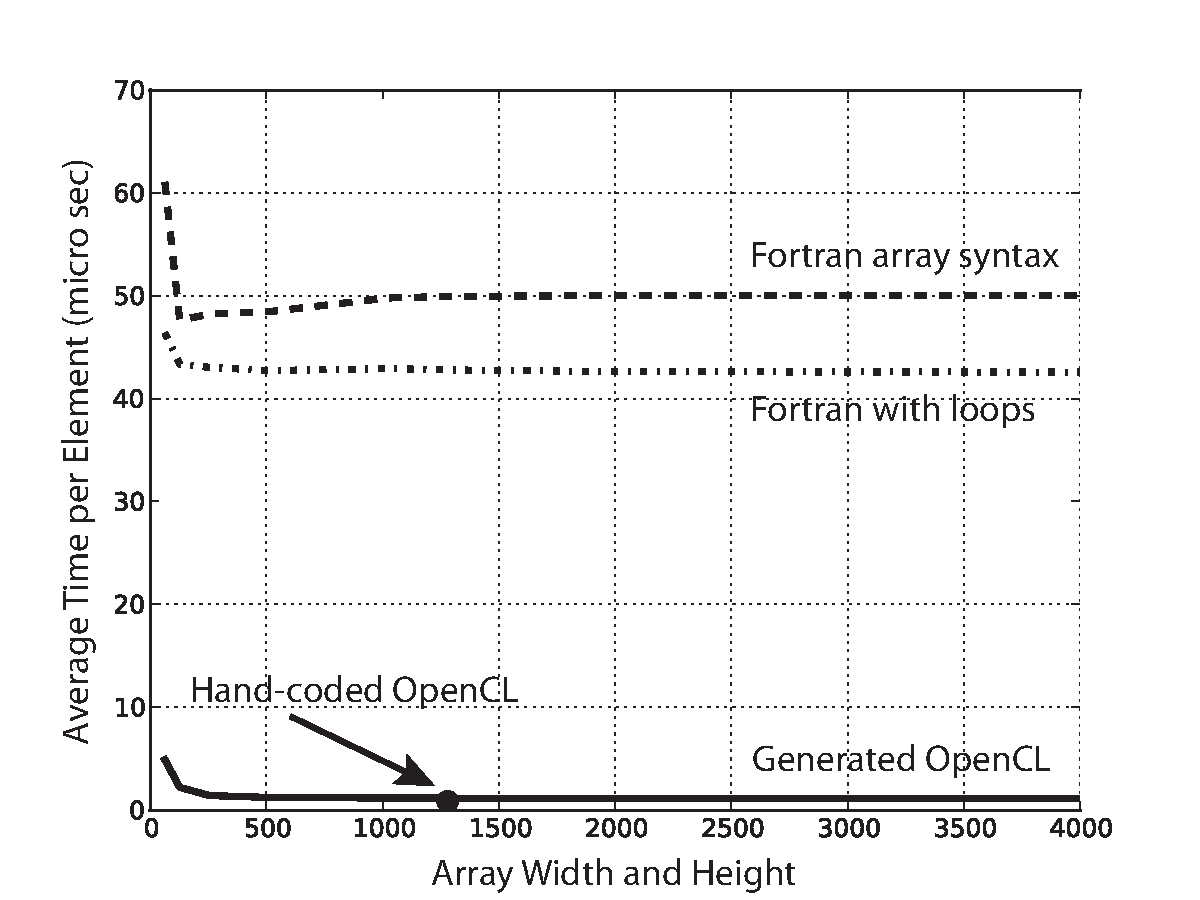
\includegraphics[width=3in]{cl-performance.pdf}
%\caption{Performance comparison for varying array size.}
%\label{fig:cl-performance}
%\end{figure}


\section{Conclusions}

Some stuff...

%%The sheer complexity of programming for clusters of many or multi-core processors with tens of millions threads of execution makes the simplicity of the data-parallel model attractive.  The increasing complexity of today's applications (especially in light of the increasing complexity of the hardware) and the need for portability across architectures make a higher-level and simpler programming model like data-parallel attractive.

%%The goal of this work has been to exploit source-to-source transformations that allow programmers to develop and maintain programs at a high-level of abstraction, without coding to a specific hardware architecture.  Furthermore these transformations allow multiple hardware architectures to be targeted without changing the high-level source.  It also removes the necessity for application programmers to understand details of the accelerator architecture or to know OpenCL.

%ACKNOWLEDGMENTS are optional
\section{Acknowledgments}
This work was supported in part by the Department of Energy Office of Science,
Advanced Scientific Computing Research.

%%TODO \cite{chamberlain04zpl, roth97stencils}

%\bibliographystyle{abbrv}
%\bibliography{local}

\balancecolumns
\end{document}
